%auteur: Amaury JOLY
\begin{frame} 
  \frametitle{Qu’est-ce qu’un relay ?} 
  \begin{itemize} 
    \item Une dApp \footnote{Decentralized Application} 
    \item Un transmetteur d’informations entre blockchains 
    \item Un suiveur d’état de chaînes connectées 
    \item Un prouveur de transactions cross-chain 
  \end{itemize} 
\end{frame}

\begin{frame} 
  \frametitle{Qu’est-ce que BTCRelay ?} 
  \begin{itemize} 
    \item Un contrat intelligent qui stocke les en-têtes de blocs Bitcoin 
    \item Un constructeur d’une mini-version de la blockchain Bitcoin 
    \item Un outil open source, sans confiance et décentralisé 
    \item Un vérificateur de transactions Bitcoin pour les contrats Ethereum 
  \end{itemize} 
\end{frame}

\begin{frame}
  \frametitle{Qu’est-ce que BTCRelay ?}
  \centering
  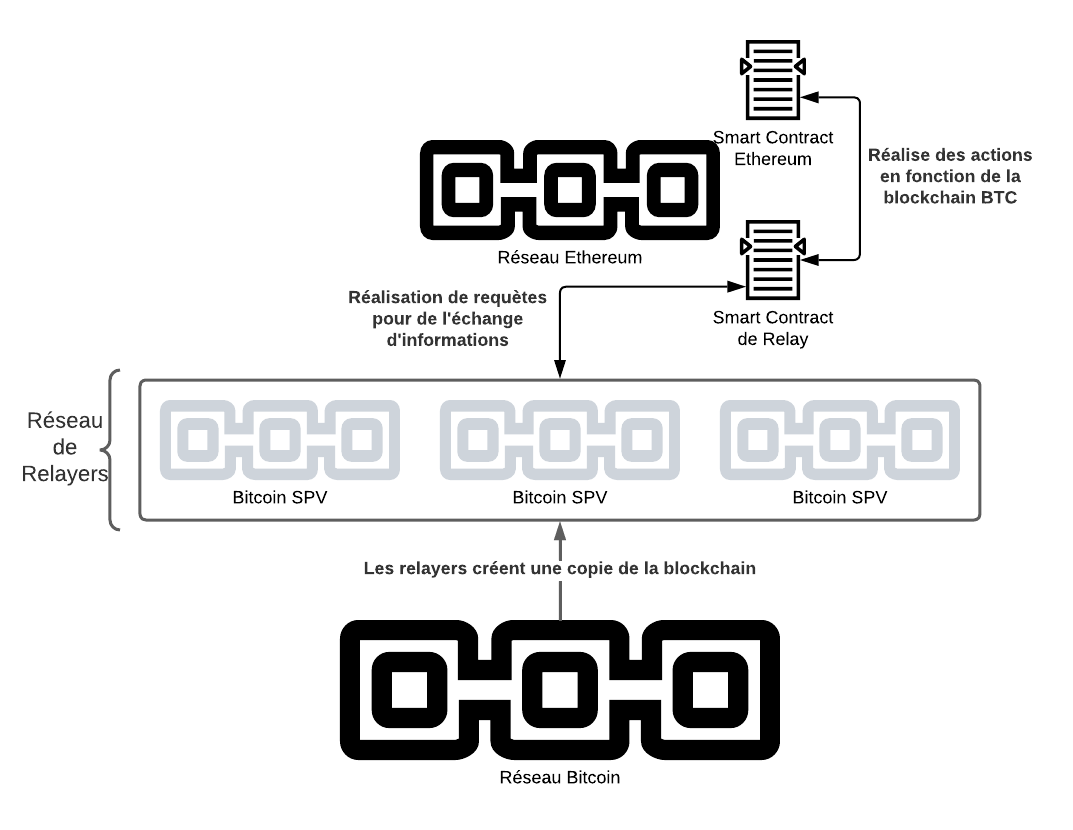
\includegraphics[scale = 0.5]{decentralisation/btcRelay.png}
\end{frame}

\begin{frame} 
  \frametitle{Qu’est-ce que tBTC ?} 
  \begin{itemize} 
    \item Un projet de relay entre Bitcoin et Ethereum 
    \item Un échangeur de bitcoins contre des tokens ERC-20 
    \item Un contrat Deposit qui interagit avec des signataires 
    \item Un utilisateur de BTCRelay pour vérifier les transactions Bitcoin 
  \end{itemize}
\end{frame}
